\subsection{Quatre cercles structurant l'action de l'IHEDN}
\label{annexe:figures_complementaires:cercles_structurants_action_IHEDN}

\begin{figure}[H]
\centering
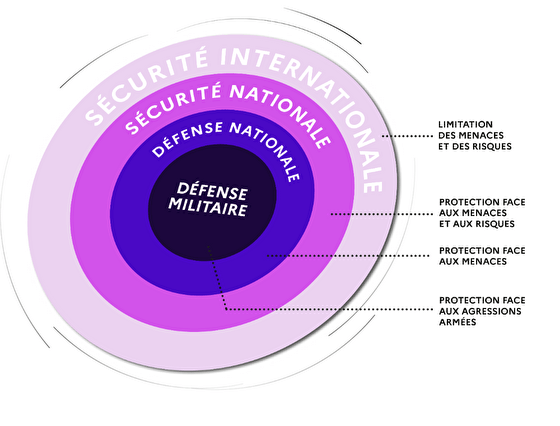
\includegraphics[width=0.8\linewidth]{Figures/cercles.png}
\caption[Quatre cercles structurant l'action de l'IHEDN]{Quatre cercles structurant l'action de l'IHEDN\footnotemark.}
\label{fig:cercles}
\end{figure}
\footnotetext{Illustration issue de : \cite{IHEDN_perimetre_defense_nationale}.}

\clearpage

\subsection{Chaîne opérationnelle de gestion de crise.}
\label{annexe:figures_complementaires:chaine_operationnelle_gestion_de_crise}

\begin{figure}[H]
\centering
\rotatebox{90}{%
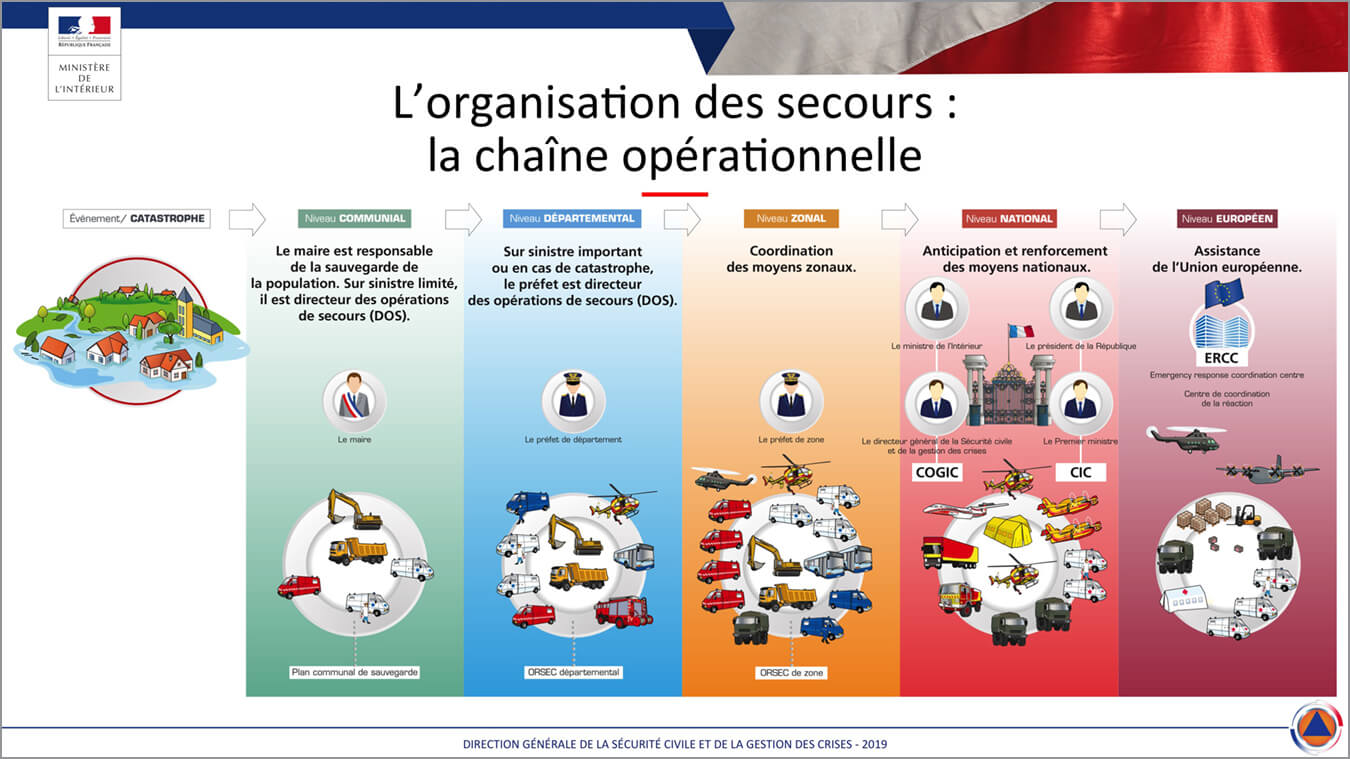
\includegraphics[width=0.82\textheight]{Figures/Chaine_operationnelle_gestion_crises.jpg}%
}
\caption[Chaîne opérationnelle de gestion de crise.]{Chaîne opérationnelle de gestion de crise\footnotemark.}
\label{fig:chaine_operationnelle}
\end{figure}

\footnotetext{Illustration issue de : \cite{dispositif_gestion_de_crise}.}

\clearpage

\subsection{Calendrier prévisionnel de mise en \oe{}uvre du questionnaire}
\label{annexe:figures_complementaires:calendrier_questionnaire}

La figure \ref{fig:gantt-questionnaire-ar16} présente l'enchaînement des différentes étapes du projet de mise en \oe{}uvre du questionnaire, depuis leur planification jusqu'à l'obtention et l'exploitation des résultats en septembre 2027.

\begin{figure}[H]
\centering
\makeatletter
\providecommand{\ganttvrulelabel}[4][]{%
  \begingroup
  \ganttset{#1}%
  \gtt@tsstojulian{#4}{\gtt@vrule@slot}%
  \gtt@juliantotimeslot{\gtt@vrule@slot}{\gtt@vrule@slot}%
  \pgfmathsetmacro\y@upper{%
    \gtt@lasttitleline * \ganttvalueof{y unit title}%
  }%
  \pgfmathsetmacro\y@lower{%
    \gtt@lasttitleline * \ganttvalueof{y unit title}%
    + (\gtt@currentline - \gtt@lasttitleline - 1)%
    * \ganttvalueof{y unit chart}%
  }%
  \pgfmathsetmacro\x@mid{%
    (\gtt@vrule@slot - 1 + \ganttvalueof{vrule offset})%
    * \ganttvalueof{x unit}%
  }%
  \pgfmathsetmacro\y@label{\y@lower - #2}%
  \draw [/pgfgantt/vrule]
    (\x@mid pt, \y@upper pt) -- (\x@mid pt, \y@label pt)
    node [/pgfgantt/vrule label node] {#3};%
  \endgroup
}
\makeatother

\begin{ganttchart}[
    hgrid,
    x unit=0.0147cm,
    y unit chart=0.58cm,
    time slot format=isodate,
    title/.style={fill=gray!20, draw=gray!60},
    title label font=\bfseries\fontsize{6.4pt}{7pt}\selectfont,
    bar label font=\fontsize{6.8pt}{7.4pt}\selectfont,
    group label font=\bfseries\fontsize{6.8pt}{7.4pt}\selectfont,
    bar height=0.60,
    group height=0.38,
    group right shift=0,
    group left shift=0,
    group peaks tip position=0,
    group peaks height=0.18,
    group peaks width=0.2,
    bar/.style={fill=gray!35, draw=gray!70},
    group/.style={fill=gray!70, draw=gray!80},
    vrule/.style={dashed, line width=0.6pt, draw=black!70},
    vrule offset=.5,
    vrule label font=\fontsize{5pt}{5.6pt}\selectfont,
    vrule label node/.append style={anchor=north, rotate=45, align=left, inner sep=0.5pt, text=black!80},
    canvas/.style={draw=gray!50},
    y unit title=0.58cm,
    title height=1,
    title label anchor/.style={below=-1.6ex},
    bar label node/.append style={text width=4.2cm, align=right},
    group label node/.append style={text width=4.2cm, align=right}
]{2025-10-01}{2027-09-30}

\gantttitle{2025}{92}
\gantttitle{2026}{365}
\gantttitle{2027}{273} \\
\gantttitle{Oct}{31}
\gantttitle{Nov}{30}
\gantttitle{Déc}{31}
\gantttitle{Jan}{31}
\gantttitle{Fév}{28}
\gantttitle{Mar}{31}
\gantttitle{Avr}{30}
\gantttitle{Mai}{31}
\gantttitle{Juin}{30}
\gantttitle{Juil}{31}
\gantttitle{Août}{31}
\gantttitle{Sep}{30}
\gantttitle{Oct}{31}
\gantttitle{Nov}{30}
\gantttitle{Déc}{31}
\gantttitle{Jan}{31}
\gantttitle{Fév}{28}
\gantttitle{Mar}{31}
\gantttitle{Avr}{30}
\gantttitle{Mai}{31}
\gantttitle{Juin}{30}
\gantttitle{Juil}{31}
\gantttitle{Août}{31}
\gantttitle{Sep}{30} \\

\ganttgroup{Cadrage stratégique}{2025-10-01}{2026-06-25} \\
\ganttbar[bar/.append style={fill=blue!35}]{Étude bibliographique}{2025-10-01}{2026-04-30} \\
\ganttbar[bar/.append style={fill=blue!25}]{Sélection des trois AR pilotes}{2026-04-01}{2026-05-31} \\
\ganttbar[bar/.append style={fill=blue!45}]{Validation institutionnelle}{2026-03-30}{2026-05-25} \\

\ganttgroup{Conception du questionnaire}{2026-02-01}{2026-12-31} \\
\ganttbar[bar/.append style={fill=green!35}]{Objectifs, problématique et thèmes}{2026-02-01}{2026-12-31} \\
\ganttbar[bar/.append style={fill=green!25}]{Trame et grille d'exploitation}{2026-06-01}{2026-12-31} \\
\ganttbar[bar/.append style={fill=green!45}]{Maquette, support et outils}{2026-06-01}{2026-08-31} \\

\ganttgroup{Mobilisation et gouvernance}{2026-07-01}{2026-12-31} \\
\ganttbar[bar/.append style={fill=orange!35}]{Comité de pilotage}{2026-07-01}{2026-09-30} \\
\ganttbar[bar/.append style={fill=orange!25}]{Comité scientifique}{2026-07-01}{2026-09-30} \\
\ganttbar[bar/.append style={fill=orange!45}]{Ressources et partenariats}{2026-07-01}{2026-09-30} \\
\ganttbar[bar/.append style={fill=green!55}]{Validation RGPD et consentement}{2026-10-01}{2026-12-31} \\
\ganttbar[bar/.append style={fill=orange!55}]{Communication projet}{2026-10-01}{2026-12-31} \\
\ganttbar[bar/.append style={fill=orange!65}]{Préparation de l'emailing}{2026-10-01}{2026-12-31} \\

\ganttgroup{Lancement et déploiement}{2027-01-04}{2027-03-31} \\
\ganttbar[bar/.append style={fill=red!30}]{Lancement du questionnaire}{2027-01-04}{2027-02-28} \\
\ganttbar[bar/.append style={fill=red!40}]{Administration et relances}{2027-02-28}{2027-03-31} \\

\ganttgroup{Exploitation et valorisation}{2027-04-01}{2027-09-15} \\
\ganttbar[bar/.append style={fill=purple!25}]{Traitement des résultats}{2027-04-01}{2027-05-31} \\
\ganttbar[bar/.append style={fill=purple!35}]{Analyse et cartographie des compétences}{2027-04-01}{2027-06-30} \\
\ganttbar[bar/.append style={fill=purple!45}]{Rédaction du rapport de travail}{2027-06-01}{2027-08-31} \\
\ganttbar[bar/.append style={fill=purple!55}]{Capitalisation et restitution}{2027-08-01}{2027-09-15}

\ganttvrulelabel[vrule/.append style={draw=blue!70!black}, vrule label node/.append style={anchor=north east}]{10}{\shortstack[l]{15/05/2026\\Validation CODIR / Bureau}}{2026-05-15}
\ganttvrulelabel[vrule/.append style={draw=blue!70!black}, vrule label node/.append style={anchor=north west}]{34}{\shortstack[l]{25/06/2026\\Restitution du rapport de comité}}{2026-06-25}
\ganttvrulelabel[vrule/.append style={draw=red!70!black}, vrule label node/.append style={anchor=north west}]{34}{\shortstack[l]{31/03/2027\\Clôture de l'enquête}}{2027-03-31}
\ganttvrulelabel[vrule/.append style={draw=purple!70!black}, vrule label node/.append style={anchor=north east}]{10}{\shortstack[l]{15/09/2027\\Restitution finale}}{2027-09-15}

\end{ganttchart}

\caption{Calendrier prévisionnel de mise en \oe{}uvre du questionnaire de cartographie des compétences des membres de l'\ARSeize.}
\label{fig:gantt-questionnaire-ar16}
\end{figure}